\chapter{Implementierung der automatisierten Testinfrastruktur}

Das Endziel dieser Arbeit ist die Einrichtung einer automatisierten
Testinfrastruktur, um die Webanwendung jExam und ihre zukünftige
Version, die sich noch in der Entwicklung befindet, zu testen.
Dabei sollen nicht nur die wichtigsten
Funktionen getestet werden, sondern auch die Sicherheit und die
Performance. Dieses Kapitel konzentriert sich auf die Einrichtung
dieser Testinfrastruktur sowie auf das Design und die Entwicklung
der Tests. Außerdem werden die verschiedenen verwendeten Technologien
vorgestellt und ihre Verwendung begründet.


\section{Vorstellung der Testansatzes}

Die jExam-Webanwendung muss auf drei verschiedenen Ebenen getestet
werden: Funktionalitäten, Performance und Sicherheit. Es ist jedoch
nicht möglich, diese drei Ebenen in einer einzigen Testsuite zu
kombinieren. Dies erfordert die Einrichtung einer Infrastruktur,
die die Erstellung und Ausführung der Tests verwaltet. Die Anwendung,
die verwendet wird, um die verschiedenen Dienste zu trennen, ist Docker \cite{docker}
(wird in den folgenden Kapiteln behandelt). Docker  wird nicht nur für
die Trennung der Testebenen verwendet. Sie ermöglicht es auch, beide
Versionen von jExam zu deployen, sodass sie effizient und lokal
getestet werden können. Über diese Infrastruktur wird es möglich
sein, Tests auszuführen und am Ende ihrer Ausführung Berichte und
Metriken zu erhalten. Über diese Infrastruktur wird es möglich sein,
Tests auszuführen und am Ende ihrer Ausführung Berichte und Metriken
zu erhalten. Diese ermöglichen , die Leistung der beiden Plattformen
zu beobachten und zu vergleichen. In den nächsten Kapiteln werden
alle diese Konzepte im Detail behandelt.


\section{Entwicklung von Sicherheitstests}

\subsection{\acs{owasp}}

\acs{owasp} ist das Akronym für \textbf{O}pen \textbf{W}eb
\textbf{A}pplication \textbf{S}ecurity \textbf{P}roject und
beschreibt eine offene Organisation, deren Hauptziel ist, die
Sicherheit von Anwendungen, Diensten und Software zu verbessern.
Sie wurde am 1. Dezember 2001 gegründet und am 21. April 2004 als
gemeinnützige Organisation offiziell anerkannt.  Sie ermöglicht
Organisationen, Unternehmen oder Einzelpersonen, sichere Anwendungen zu
entwickeln und zu warten. Die \acs{owasp} hat eine Reihe von
Sicherheitstools und -richtlinien entwickelt. Dazu gehören die \acs{owasp}
Top 10 und der Zed Attack Proxy (\acs{zap}). Ein wichtiger
Grundsatz der OWASP ist, dass jeder, der sich für die Sicherheit
von Webanwendungen interessiert, weltweit kostenlos über das
nötige Wissen und die Werkzeuge verfügen kann (vgl. \cite{owasp}).
In diesem Zusammenhang hat sie die OWASP TOP 10 erstellt, die eine
Liste der zehn häufigsten Sicherheitslücken im Internet
darstellt. Ihr Hauptzweck ist die Schulung all jener, die mit der
Entwicklung sicherer Anwendungen zu tun haben.  Sie sollen über die
üblichsten Sicherheitslücken informiert werden und dadurch diese
vermeiden.  Im Folgenden werden die zehn Angriffe der OWASP TOP
10 auf der Basis der OWASP TOP 10 2017 
Release Candidate 2 (vgl. \cite{Stock2017}) beschrieben.

\begin{table}[h]
    \begin{tabulary}{\textwidth}{@{}L@{}}
        \toprule
        \textbf{OWASP TOP10 2017} \tabularnewline\midrule
        1"~ Injektion (Injection)
        \tabularnewline
        2"~ Fehler in der Authentifizierung (Broken Authentication)
        \tabularnewline
        3"~ Verlust der Vertraulichkeit von Daten (Sensitive Data Exposure)
        \tabularnewline
        4"~ XML External Entities (XML)
        \tabularnewline
        5"~ Fehler in der Zugriffskontrolle (Broken Access Control)
        \tabularnewline
        6"~ Sicherheitsrelevante Fehlkonfiguration (Security Misconfiguration)
        \tabularnewline
        7"~ Cross-Site-Scripting (XSS)
        \tabularnewline
        8"~ Unsichere Deserialisierung (Insecure Deserialization)
        \tabularnewline
        9"~ Nutzung von Komponenten mit bekannten Schwachstellen (Using Components with Known Vulnerabilities)
        \tabularnewline
        10"~ Unzureichendes Logging und Monitoring (Insufficient Logging and Monitoring)
        \tabularnewline\bottomrule
    \end{tabulary}
    \caption{OWASP TOP 10 2017}\label{tab:OWASP_TOP_10}
\end{table}

\subsubsection{Injektion}

Eine Injektion ist eine Schwachstelle, die einem Angreifer ermöglicht,
bösartigen Code durch eine Anwendung auf ein anderes System zu
schleusen. Dabei können sowohl Backend-Systeme als auch andere
Clients, die mit der angreifbaren Anwendung verbunden sind, gefährdet
werden. Zu den Auswirkungen dieser Angriffe gehören:

\begin{enumerate}
    \item Einem Angreifer erlauben, Betriebssystemaufrufe auf einem
    Zielrechner auszuführen.
    \item Einem Angreifer ermöglichen, Backend-Datenspeicher
    zu kompromittieren.
    \item Einem Angreifer ermöglichen, die Sitzungen anderer
    Benutzer zu kompromittieren oder umzuleiten.
    \item Einem Angreifer erlauben, Aktionen im Namen anderer
    Benutzer oder Dienste zu erzwingen.
\end{enumerate}

Viele Webanwendungen hängen von Betriebssystemfunktionen, externen
Programmen und der Verarbeitung von Datenabfragen ab, die von
Benutzern eingereicht werden. Wenn eine Webanwendung Informationen
aus einer HTTP-Anfrage als Teil einer externen Anfrage weitergibt,
sollten Sie eine Möglichkeit zur Überprüfung und Validierung der
Nachricht einrichten. Andernfalls kann ein Angreifer spezielle
(Meta-) Zeichen, bösartige Befehle/Codes oder Befehlsmodifikatoren in
die Nachricht einfügen. Diese Angriffe sind zwar nicht schwer
auszuführen, aber es gibt immer mehr Tools, die nach diesen
Fehlern suchen. Ein Angreifer kann diese Techniken nutzen, um den
Inhalt Ihrer Datenbank zu erhalten, zu beschädigen oder zu zerstören,
Backend-Systeme zu kompromittieren oder andere Benutzer anzugreifen.
Erfolgreiche Injektionsangriffe können ein System vollständig
gefährden oder zerstören. Es ist wichtig, auf diese Arten von
Angriffen zu testen und sich dagegen zu schützen.

Als Beispiel kann man die SQL-Injektion nennen. Diese ist eine
besonders weit verbreitete und gefährliche Form der Injektion.
Um einen SQL-Injektion-Fehler auszunutzen, muss ein Angreifer
einen Parameter finden, den die Webanwendung an eine
Datenbankinteraktion weitergibt. Ein Angreifer kann dann
bösartige SQL-Befehle in den Inhalt des Parameters einbetten.
Das bringt die Webanwendung dazu, eine bösartige Abfrage an die
Datenbank weiterzuleiten. SQL-Abfragen könnten durch Hinzufügen
zusätzlicher ``Einschränkungen'' zu einer Anweisung (z. B. OR 1=1)
geändert werden, um Zugriff auf nicht autorisierte Daten zu
erhalten oder diese zu ändern.



\subsubsection{Fehler in der Authentifizierung}

Wenn die Authentifizierungsfunktionen  einer Anwendung nicht korrekt
implementiert sind, können Angreifer Passwörter oder Sitzungs-IDs
kompromittieren oder andere Implementierungsfehler ausnutzen, indem
sie die Anmeldedaten anderer Benutzer verwenden. Diese Schwachstelle
wird als ``Fehler in der Authentifizierung'' (Broken authentication
in Englisch) bezeichnet. Es wird in der Regel durch schlecht
implementierte Authentifizierungs- und Sitzungsverwaltungsfunktionen
verursacht. In diesem Fall  zielen Angriffe darauf ab, die Kontrolle
über ein oder mehrere Benutzerkonten zu erlangen, indem der Angreifer
die gleichen Privilegien erhält wie der angegriffene Benutzer.
Es wird vom ``Fehler in der Authentifizierung'' besprochen ,
wenn Angreifer in der Lage sind, Passwörter, Schlüssel oder
Sitzungs-Tokens, Benutzerkontoinformationen und andere
Details zu kompromittieren, um Benutzeridentitäten zu übernehmen.
Zu den üblichen Risikofaktoren gehören:


\begin{enumerate}
    \item Vorhersehbare Anmeldekennungen
    \item Benutzerauthentifizierungskennungen, die nicht geschützt sind, wenn sie gespeichert werden.
    \item Sitzungs-IDs, die in der URL offengelegt werden (z. B. durch URL-Rewriting).
    \item Sitzungs-IDs, die anfällig für Session-Fixing-Angriffe sind.
    \item Sitzungswert, der nach dem Abmelden nicht unterbrochen oder ungültig gemacht wird.
    \item Sitzungskennungen, die nach einer erfolgreichen Anmeldung nicht erneuert werden.
    \item Passwörter, Sitzungskennungen und andere Identifikationsinformationen, die über unverschlüsselte Verbindungen gesendet werden.
\end{enumerate}
\subsubsection{Verlust der Vertraulichkeit von Daten}

Der Verlust der Vertraulichkeit von  Daten tritt auf, wenn eine
Organisation unwissentlich sensible Daten offenlegt oder wenn ein
Sicherheitsvorfall dazu führt, dass sensible Daten versehentlich
oder rechtswidrig zerstört, verloren, verändert, unbefugt
offengelegt oder unbefugt darauf zugegriffen wird. Eine solche
Datenexposition kann das Ergebnis eines unzureichenden Schutzes einer
Datenbank, einer Fehlkonfiguration bei der Erstellung neuer Instanzen
von Datenspeichern oder einer unsachgemäßen Nutzung von Datensystemen sein.

Klassische Beispiele dafür sind in Klartext gespeicherte Daten, wie
Passwörter oder Kreditkartendaten, fehlendes HTTPS auf
authentifizierten Webseiten, und Hash-Passwörter, die ohne zugefügtes
“Salz” erstellt wurden. Salz bezeichnet eine zufällige Zeichenfolge,
die den Klardaten vor der Verschlüsselung hinzugefügt werden. Dadurch
kann anhand identischer Hashwerte nicht darauf geschlossen werden,
dass es sich um dieselben Daten handelt.
\subsubsection{XML External Entities (XML)}

\acs{xml} External Entity Injection (auch bekannt als \acs{xee}) ist eine
Sicherheitslücke, die einem Angreifer ermöglicht, in die Verarbeitung
von \acs{xml}-Daten durch eine Anwendung einzugreifen. Dieser Angriff
erfolgt, wenn die \acs{xml}-Eingabe, die einen Verweis auf eine externe
Entität enthält, von einem schwach konfigurierten \acs{xml}-Parser
verarbeitet wird. Dieser Angriff kann zur Offenlegung vertraulicher
Daten, Denial of Service, serverseitiger Anfragefälschung,
Portanalyse aus der Sicht des Computers, auf dem sich der Parser
befindet, und anderen Auswirkungen auf das System führen. Um \acs{xxe}
Injections zu verhindern, sollen folgende Punkte beachtet werden:


\begin{enumerate}
    \item Einfachere Datenformate wie JSON zur Datenübertragung verwenden.
    \item Das Verbot in allen \acs{xml}-Parsern, \acs{xml}-Entitäten
     und \acs{dtd}s verändern. \acs{dtd} steht für Document Type Definition und
     bezeichnet einen XML Dokument, in welchem XML-Entities
     definiert werden. Auf dieser Weise wird vermieden,
     dass ein Benutzer eigenen Entities erstellt.
    \item Deaktivierung des Hochladens von XML-Dateien
\end{enumerate}

\subsubsection{Fehler in der Zugriffskontrolle}

Fehler in der Zugriffskontrolle ist eine Sicherheitslücke,
die es Angreifern ermöglicht, Berechtigungsgarantien zu
umgehen und Tätigkeiten auszuführen, als wären sie
privilegierte Benutzer.

Die Zugriffskontrolle sorgt dafür, dass Benutzer nicht
außerhalb der ihnen zugewiesenen Befugnisse handeln
können. Fehler führen in der Regel zur unbefugten
Offenlegung von Informationen, zur Änderung oder Zerstörung
aller Daten oder zur Ausführung einer Geschäftsfunktion
außerhalb der Grenzen des Benutzers. Häufige Schwachstellen
bei der Zugriffskontrolle sind:

\begin{enumerate}
    \item Umgehung von Zugriffskontrollprüfungen durch
    Änderung der URL, des internen Anwendungsstatus oder
    der HTML-Seite oder einfach durch Verwendung eines
    benutzerdefinierten API-Angriffstools.

    \item Ermöglichung der Änderung des Primärschlüssels
    in den Datensatz eines anderen Benutzers, wodurch
    die Anzeige oder Bearbeitung des Kontos eines anderen
    Benutzers ermöglicht wird.

    \item Ausweitung der Rechte. Als Benutzer handeln, ohne
    eingeloggt zu sein, oder als Administrator handeln, wenn
    man als Benutzer eingeloggt ist.

    \item Manipulation von Metadaten, wie z. B. die
    Wiedergabe oder Manipulation eines JSON Web Token
    (JWT)-Zugangskontrolltokens oder eines Cookies oder
    eines versteckten Feldes, das manipuliert wurde, um
    die Privilegien zu erhöhen, oder der Missbrauch der
    JWT-Ungültigkeitserklärung.

    \item CORS-Fehlkonfiguration ermöglicht
    nicht autorisierten API-Zugriff.

    \item Erzwingen des Navigierens auf authentifizierten
    Seiten als nicht authentifizierter Benutzer oder
    auf privilegierten Seiten als Standardbenutzer.
    Zugriff auf API mit fehlenden Zugriffskontrollen
    für POST, PUT und DELETE.
\end{enumerate}

\subsubsection{Sicherheitsrelevante Fehlkonfiguration}

Sicherheitsrelevante Fehlkonfigurationen sind 
Sicherheitskontrollen, die ungenau konfiguriert oder
unsicher sind. Dadurch werden Ihre Systeme und Daten 
gef\"ahrdet. Grunds\"atzlich kann jede schlecht dokumentierte 
Konfigurations\"anderung, Standardeinstellung oder ein 
technisches Problem bei einer beliebigen Komponente zu 
einer Fehlkonfiguration f\"uhren.

Eine Fehlkonfiguration kann aus einer Vielzahl von 
Gr\"unden auftreten. Moderne Netzwerkinfrastrukturen sind
\"au{\ss}erst komplex und zeichnen sich durch st\"andige
Ver\"anderungen aus. Organisationen k\"onnen leicht 
entscheidende Sicherheitseinstellungen \"ubersehen, 
insbesondere bei neuen Netzwerkger\"aten, die 
Standardkonfigurationen beibehalten k\"onnen. Wenn
sichere Konfigurationen f\"ur Zugangspunkte eingerichtet 
werden, m\"ussen Konfigurationen mit Sicherheitskontrollen
h\"aufig \"uberpr\"uft werden, um unvermeidliche 
Konfigurationsabweichungen zu erkennen. Systeme
\"andern sich, neue Ger\"ate werden in das Netzwerk
eingef\"uhrt, Patches werden eingespielt - all dies
tr\"agt zu fehlerhaften Konfigurationen bei.


\subsubsection{Cross-Site-Scripting (XSS)}


\subsection{ZAP Proxy}

Wie in \autoref{ch:sicherheit} erwähnt, müssen beide Versionen von jExam
auf größere Sicherheitslücken gescannt werden. Schwachstellen-Scanner für
Webanwendungen sind automatisierte Tools, die Webanwendungen - normalerweise
von außen - auf Sicherheitslücken wie Cross-Site-Scripting, SQL Injektion,
Command Injektion, Path Traversal und unsichere Serverkonfiguration
untersuchen (vgl. \cite{vulscan}). Diese Kategorie von Tools wird häufig
als Dynamic Application Security Testing (\acs{dast}) Tools bezeichnet.
Es gibt eine große Anzahl kommerzieller und Open-Source-Tools dieser Art,
und alle diese Tools haben ihre eigenen Stärken und Schwächen. Die Analyse
der verschiedenen Tools zum Aufspüren von Schwachstellen wird in dieser
Arbeit nicht behandelt. Es gibt jedoch das OWASP Benchmark-Projekt
(vgl \cite{benchmark}), das die Effektivität aller Arten von Tools zum
Aufspüren von Schwachstellen, einschließlich \asc{dast}, wissenschaftlich
misst. Das Tool zum Scannen von Schwachstellen, das in dieser Arbeit verwendet wird,
ist ZAP Proxy.

\acs{zap} steht für Zed Attack Proxy und bezeichnet eine
Open-Source-Sicherheitssoftware, die in der Programmiersprache Java
geschrieben und 2010 veröffentlicht wurde. Sie wird verwendet, um
Webanwendungen auf Schwachstellen zu scannen. Es wurde als kleines
Projekt vom Open Web Application Security Project (OWASP) gestartet und
ist heute das aktivste Projekt, das von Tausenden von Menschen auf der
ganzen Welt betreut wird. Es ist der am häufigsten verwendete
Webanwendungsscanner (vgl. \cite{zap}). \acs{zap} ist für Linux, Windows und Mac
in 29 Sprachen verfügbar. Zed Attack Proxy wird verwendet, um
Schwachstellen auf beliebigen Webservern zu erkennen. Zu den wichtigsten
Schwachstellen, die von \asc{zap} erkannt werden können, gehören :

\begin{enumerate}
    \item SQL injektion (Injection)
    \item Fehler in der Authentifizierung (Broken Authentication)
    \item Verlust der Vertraulichkeit von Daten (Sensitive data exposure)
    \item Fehler in der Zugriffskontrolle (Broken Access control)
    \item Sicherheitsrelevante Fehlkonfiguration (Security misconfiguration)
    \item Cross Site Scripting (XSS)
    \item Unsichere Deserialisierung (Insecure Deserialization)
    \item Nutzung von Komponenten mit bekannten Schwachstellen (Components with known vulnerabilities)
    \item Fehlende Sicherheitsheader (Missing security headers)
\end{enumerate}

Was Zap zum meistgenutzten Werkzeug für Sicherheitsprüfungen macht,
ist in erster Linie die Tatsache, dass es nicht nur für die Verwendung
durch erfahrene Penetrationstester, sondern auch für Anfänger auf diesem
Gebiet konzipiert wurde. ZAP ist ein kostenloses Open-Source-Tool, das
einfach einzurichten und zu verwenden ist. Da es von einer breiten Community
verwendet wird, gibt es online im ZAP-Blog und in anderen Artikeln eine Menge
Hilfe, die Ihnen bei der Einrichtung und Verwendung des Tools hilft.
ZAP kann in einem Docker-Container ausgeführt werden. Außerdem ist die
Funktionalität skalierbar mit vielen verschiedenen Erweiterungen, die
auf GitHub veröffentlicht wurden.


ZAP ist ein so genannter "Man-in-the-middle-Proxy". Er wird zwischen den
Browser und die Webanwendung geschaltet. Während der Tester durch alle
Funktionen der Website navigiert, erfasst er alle Aktionen. Anschließend
greift er die Website mit bekannten Techniken an, um Sicherheitslücken zu
finden.  ZAP ist ein Werkzeug, das menschliche Intelligenz benötigt,
um richtig eingesetzt zu werden (es ist manuelles Werkzeug).
Penetrationstester verwenden es zunächst, um automatisch nach Schwachstellen
in einer Webanwendung zu scannen. Sobald sie eine Schwachstelle gefunden
haben, die sie ausnutzen können, verwenden sie ZAP, um die Anwendung
anzugreifen. Wie bereits in \autoref{ch:sicherheit} erwähnt, ist die einzige Funktion,
die jExam verwenden wird, der Scanner. Es geht darum, die Anwendung zu
scannen, um größere Sicherheitslücken zu finden.  Wenn die Anwendung solche
Lücken enthält, ist es für die Entwickler unerlässlich, zu handeln und
herauszufinden, wie man sie beheben kann. Auf diese Weise ist es möglich,
ZAP vollautomatisch zu verwenden.


\begin{figure}[H]
    \centering
    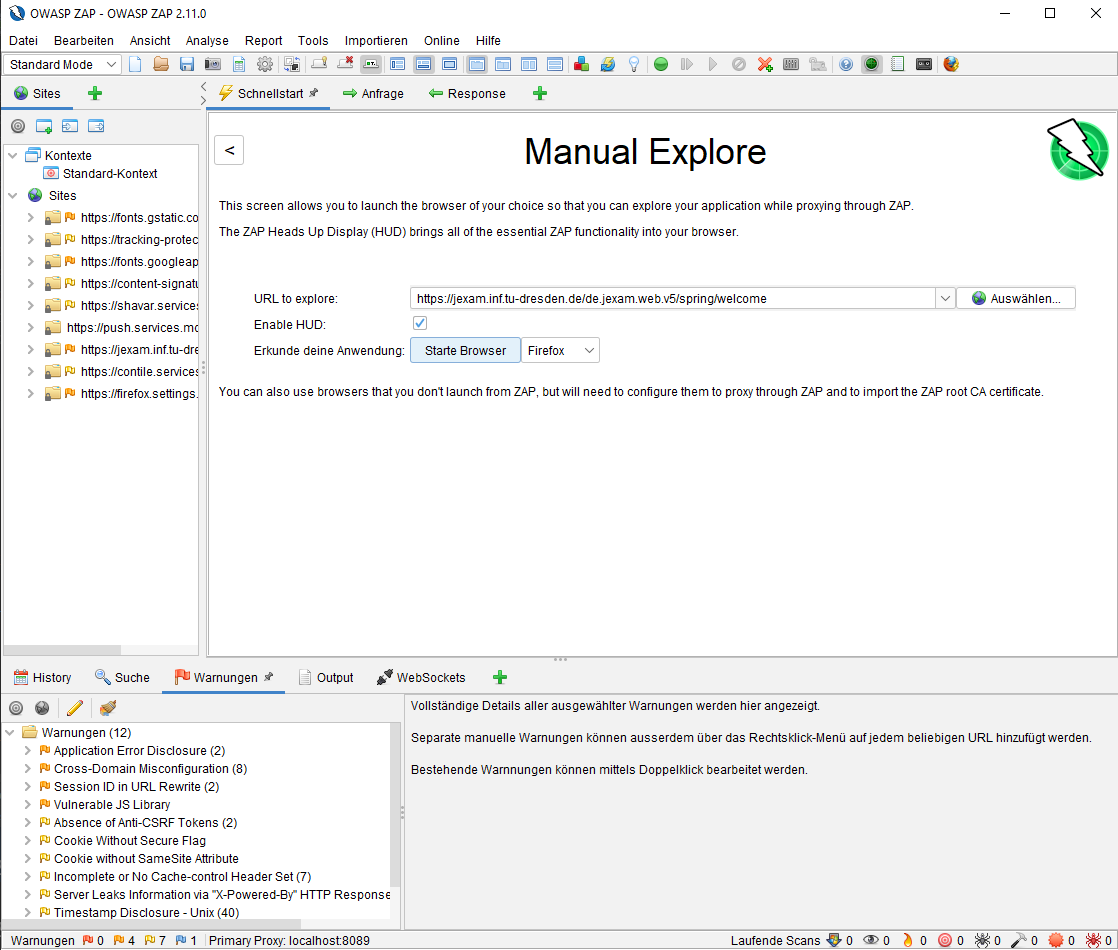
\includegraphics[scale=0.5]{images/zap-interface}
    \caption{Grafische Benutzeroberfläche von Zap} \label{fig:zap-interface}
\end{figure}



\subsection{Tests und Ergebnisse}

Die Testinfrastruktur von jExam wurde mit Docker unter Verwendung
von docker-compose entwickelt. Dies bietet die Möglichkeit, die
Testdienste in verschiedene Container aufzuteilen (dieses Konzept
wird in den nächsten Kapiteln ausführlich behandelt). Zu den
Testdiensten gehört auch ein Container, der speziell für Sicherheitstests
vorgesehen ist und automatisch bestimmte Befehle ausführt, um eine Version
von jExam zu scannen. Zunächst ist es notwendig, einige Begriffe zu
erklären, die im Folgenden verwendet werden.

\subsubsection{ZAP Spider}

Der Spider ist ein Werkzeug, das dazu dient, automatisch neue
Ressourcen (URLs) auf einer bestimmten Seite zu entdecken.
Er beginnt mit einer Liste von zu besuchenden URLs, den
sogenannten Seeds, die davon abhängen, wie der Spider gestartet
wird. Der Spider besucht dann diese URLs, identifiziert alle
Hyperlinks auf der Seite und fügt sie der Liste der zu besuchenden
URLs hinzu, und der Prozess wird rekursiv fortgesetzt, solange neue
Ressourcen gefunden werden (vgl. \cite{spider}). Dieser Prozess kann
Stunden dauern, je nachdem, wie viele Seiten und Links die Website
hat. Aus diesem Grund wird er oft mit einer Zeitbegrenzung durchgeführt.

\subsubsection{\acs{ajax} Spider}

Der \acs{ajax} Spider ist ein Add-on für einen Crawler namens Crawljax.
Das Add-on richtet einen lokalen Proxy in ZAP ein, um mit Crawljax
zu kommunizieren. Mit dem \acs{ajax} Spider ist es möglich Webanwendungen,
die  \acs{ajax} benutzen, in weit größerer Tiefe \Gls{crawlen} (Prozess der
automatischen Entdeckung neuer Ressourcen in einer Anwendung) als mit
dem nativen Spider. \acs{ajax} ist eine Reihe von Webentwicklungstechniken, die
verschiedene Webtechnologien auf der Client-Seite verwenden, um
asynchrone Webanwendungen zu erstellen. Mit \acs{ajax} können Webanwendungen
asynchron (im Hintergrund) Daten von einem Server senden und abrufen,
ohne die Anzeige und das Verhalten der bestehenden Seite zu beeinträchtigen.
Diese Computerarchitektur ermöglicht den Aufbau von Webanwendungen und
dynamischen, interaktiven Webseiten.\acs{ajax} spider wird beim Testen von Webanwendungen
empfohlen, die \acs{ajax} nutzen. Für eine vollständige Abdeckung einer
Webanwendung (z. B. um HTML-Kommentare abzudecken) soll auch den
nativen Spider verwendet werden (vgl. \cite{ajax}).

\subsubsection{Passive Scanning}

Passive Scanning ist eine Methode zur Erkennung von Schwachstellen, die auf
Informationen basiert, die aus Netzwerkdaten gesammelt werden. Beim Sammeln
dieser Informationen gibt es keine direkte Interaktion mit der Zielanwendung
(deshalb passiv). Beim passiven Scannen wird der gesamte Datenverkehr zwischen
dem Browser und der Website gelesen und aufgezeichnet, d. h. die POSTs/GETs
und ihre Antworten. ZAP analysiert diese Daten und sucht in seiner
Angriffsbibliothek nach bekannten Problemen. Passives Scannen führt keine
Angriffe aus und wird daher als harmlos angesehen. Beim passiven Scannen
können viele mögliche Fehler und Schwachstellen in einer Webanwendung
entdeckt werden.  Zu den bekanntesten gehören :

\begin{enumerate}
    \item Cross Domain Script Inclusion
    \item Cross Domain Misconfiguration
    \item X-Debug-Token Information Leak
    \item Username Hash Found
    \item Insecure Authentication
    \item Information Disclosure: Suspicious Comments
    \item Information Disclosure: Referrer
    \item Information Disclosure: In URL
    \item Information Disclosure: Debug Errors
    \item CSRF Countermeasures
\end{enumerate}

Diese Sicherheitslücken werden in dieser Arbeit nicht näher erläutert.
Informationen zu diesen Sicherheitslücken sind jedoch auf der Website von Zap Proxy
zu finden (vgl. \cite{passiv}).
\subsubsection{Active Scanning}

Active Scanning ist eine Methode zur Erkennung von Schwachstellen, bei
der versucht wird, potenzielle Schwachstellen mithilfe bekannter Angriffe
auf ausgewählte Ziele zu finden. Im Gegensatz zum passiven Scanning ist es
nicht risikolos. Es kann potenziell zu schwerwiegenden Problemen auf einem
Webserver führen. Aus diesem Grund wird Testern empfohlen, es nur für ihre
eigenen Anwendungen zu verwenden. Active Scanning ermöglicht es, mehrere
große Sicherheitslücken zu entdecken, die in einer Anwendung vorhanden
sein können. Zu den bekanntesten gehören :

\begin{enumerate}
    \item SQL Injection
    \item Directory Browsing
    \item CRLF Injection
    \item Cross Site Scripting (persistent und Reflected)
    \item Command Injection
    \item .htaccess Information Leak
\end{enumerate}

Es gibt auch viele andere, die in dieser Arbeit nicht behandelt werden.
Informationen zu diesen Sicherheitslücken sind jedoch auf der Website
von Zap Proxy zu finden (vgl. \cite{activ}).




Auf der jExam-Plattform wurden zwei Skripte für ihre Ausführung
implementiert. Es handelt sich dabei um die Skripte ZAP Baseline und
ZAP Full scan.  Da es zwei Versionen von jExam gibt, muss bei der
Ausführung der Skripte entschieden werden, welche der beiden Plattformen
getestet werden soll.

\subsubsection{ZAP Baseline}

Dieses Skript führt zuerst einen ZAP-Spider und dann ein Passiv Scanning
anhand der Daten aus dem Spider aus. Dies ist ein schneller und gründlicher
Prozess, der es ermöglicht, schnell zu erkennen, ob es ernsthafte
Schwachstellen gibt, die leicht ausgenutzt werden können. Schließlich erstellt
das Skript einen Bericht (siehe \Cref{fig:baseline}), der von den Testern sorgfältig geprüft werden muss.
Das Skript führt keinen echten ``Angriff'' durch und läuft nur für eine
relativ kurze Zeit (höchstens ein paar Minuten).


\begin{lstlisting}[language=Dockerfile,label={lst:baseline},caption={ZAP Baseline Ausführungsbefehl}]
command: [ "./wait-for-it.sh", "web:8080", "bash" ,"-c",
"zap-baseline.py -t http://web:8080 -r owaspReport.html" ]

# Web:8080: URL der Neuen Version von jExam, die sich im
Container namens Web befindet.
# ./wait-for-it.sh: Script, das einen Healt-Check
ausführt, um herauszufinden, ob die parametrisierte
Anwendung (In diesem Fall Web:8080) bereits gestartet ist.
# owaspReport.html: Webseite, die am Ende
der Testdurchführung generiert wird.
\end{lstlisting}

\subsubsection{ZAP Fullscan}


Dieses Skript führt einen ZAP Spider für eine unbestimmte Zeit aus.
Je mehr Ressourcen und Hyperlinks die Anwendung besitzt, desto länger
dauert dieser Prozess. Danach wird ein Ajax Spider ausgeführt, der
ebenfalls für eine unbestimmte Zeit ausgeführt wird. Danach wird ein
Full Active Scan ausgeführt und schließlich ein Bericht erstellt
(siehe \Cref{fig:baseline}),auf  den der Tester zugreifen kann.
Das Skript führt echte "Angriffe" aus  und kann potenziell über einen
längeren Zeitraum (mehrere Stunden) laufen. Das Skript ist jedoch viel
effizienter und findet mehr  Sicherheitslücken als ZAP Baseline.

\begin{lstlisting}[language=Dockerfile,label={lst:fullscan},caption={ZAP Fullscan Ausführungsbefehl}]
command: [ "./wait-for-it.sh", "web:8080", "bash" ,"-c",
"zap-full-scan.py -d -j -m 1 -t http://web:8080 -r owaspReport.html" ]

\end{lstlisting}


\begin{figure}[H]
    \centering
    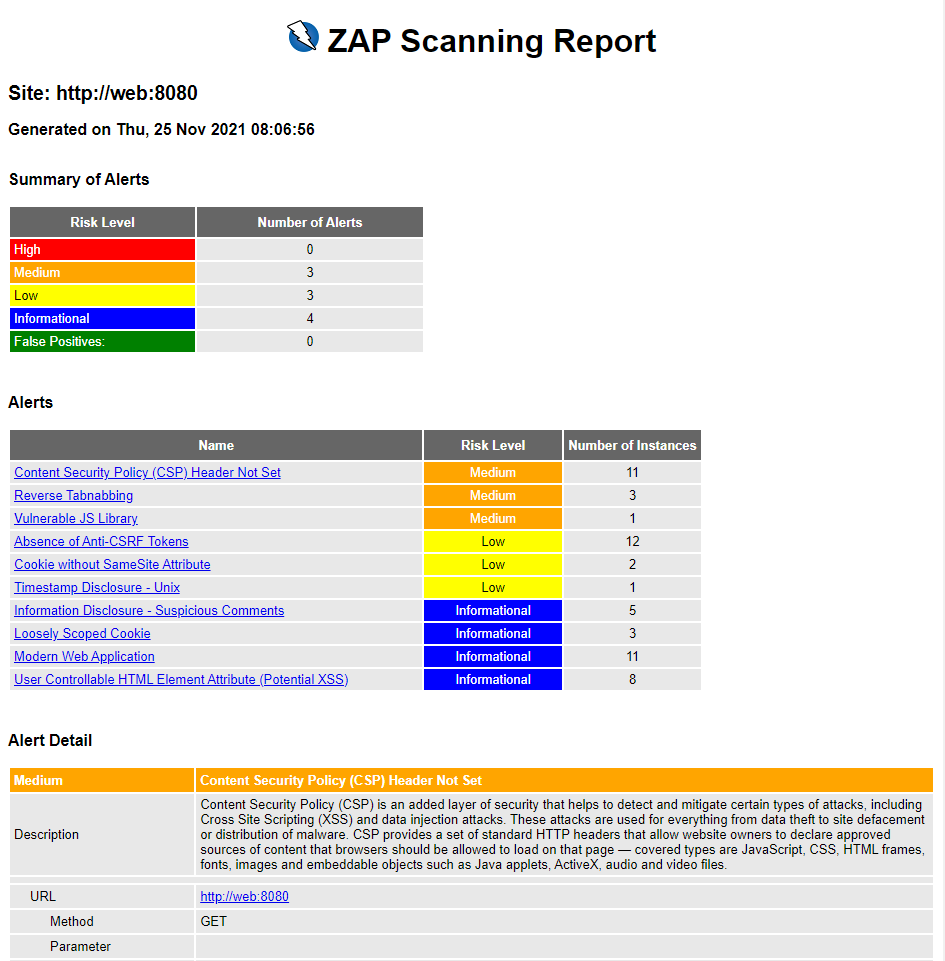
\includegraphics[scale=0.5]{images/zap-report}
    \caption{Bericht nach der Ausführung einer Zap Baseline} \label{fig:baseline}
\end{figure}




Die Sicherheit einer Anwendung zu testen ist eine schwierige Aufgabe,
aber Werkzeuge wie Zap machen die Tür zu diesem Bereich der Programmierung
immer kleiner. Mit Hilfe der Scanner ist es möglich, Sicherheitslücken zu
finden, die den Entwicklern ermöglichen, sie zu beheben. Dadurch wird eine
gute Softwarequalität für die Zukunft gewährleistet.









\section{Entwicklung von Performancetests}
\section{Entwicklung von UI-Tests}


Die Entwicklung von UI-Tests ist der zentrale Punkt dieser Arbeit. Im
Gegensatz zu Performance- und Sicherheitstests, die nicht funktional sind,
ist das Hauptziel dieser UI-Tests festzustellen, ob die beiden Versionen von
jExam so funktionieren, wie die Entwickler es beabsichtigt haben.
Dieses Kapitel konzentriert sich auf die Entwicklung der UI-Tests, die
verschiedenen Tools und die Design Patterns, die verwendet wurden. Zunächst
werden die verschiedenen Werkzeuge vorgestellt, die bei der Entwicklung
verwendet wurden. Anschließend werden die Design Patterns vorgestellt, die
dabei helfen, den Code robust und leicht wartbar zu machen. In Teil drei
wird der Schwerpunkt auf die Implementierung von Tests gelegt, und im letzten
Teil werden die erzielten Ergebnisse und zusätzliche Funktionen vorgestellt.

\subsection{Verwendete Werkzeuge}

\subsubsection{Selenium Webdriver}

Selenium ist ein Open-Source-projekt für eine Reihe von Tools und Bibliotheken
zur Unterstützung der Webbrowser-Automatisierung (vgl. \cite{selenium-survey}).
Selenium bietet  Werkzeuge zur Erstellung funktionaler Tests, ohne dass eine
Testskriptsprache erlernt werden muss. Außerdem bietet es eine testspezifische
Sprache (Selenese), mit der Tests in einer Reihe beliebter Programmiersprachen
geschrieben werden können, darunter JavaScript (Node.js), C#, Groovy, Java,
Perl, PHP, Python, Ruby und Scala. Die Tests können dann mit den meisten
modernen Webbrowsern ausgeführt werden. Selenium läuft auf Windows, Linux
und macOS. Selenium besteht aus mehreren Komponenten, von denen jede eine
bestimmte Rolle bei der Entwicklung der Testautomatisierung von Webanwendungen
übernimmt. Zu diesen Komponenten gehören: die Selenium IDE, Selenium Client API,
Selenium Remote Control, Selenium Grid und schließlich der Selenium WebDriver,
der in dieser Arbeit verwendet wird.

Das Kernelement von Selenium ist Selenium WebDriver, eine Schnittstelle zum
Schreiben von Anweisungen, die in verschiedenen Browsern austauschbar sind.
Selenium WebDriver nimmt Befehle entgegen (die in \gls{selenese} oder über eine
Client-API gesendet werden) und sendet sie an einen Browser. Dies wird durch
einen browserspezifischen Browsertreiber implementiert, der Befehle an einen
Browser sendet und Ergebnisse abruft. Die meisten Browsertreiber starten
tatsächlich eine Browseranwendung (z. B. Firefox, Google Chrome, Internet
Explorer, Safari oder Microsoft Edge) und greifen darauf zu. Selenium WebDriver
benötigt keinen speziellen Server, um Tests auszuführen. Stattdessen startet
der WebDriver direkt eine Browserinstanz und steuert sie.  Wo immer möglich,
verwendet WebDriver native Funktionen auf Betriebssystemebene und nicht
browserbasierte JavaScript-Befehle zur Steuerung des Browsers. Dadurch werden
Probleme mit subtilen Unterschieden zwischen nativen und JavaScript-Befehlen,
einschließlich Sicherheitseinschränkungen, vermieden (vgl. \cite{Stewart2016}).
Selenium WebDriver ist vollständig implementiert und wird in JavaScript
(Node.js), Python, Ruby, Java, Kotlin und C# unterstützt.


Selenium ist derzeit das von Testern am meisten geliebte Framework für
UI-Testing (vgl. \cite{selenium-survey} , S. 08-09). Es hat viele Vorteile,
wie z.B. die \"Ubertragbarkeit auf alle Systeme, die einfache Integration mit
andere Technologien, eine große und dynamische Entwicklergemeinschaft sowie
die Dokumentation und die Fülle an verfügbaren Ressourcen. Im Rahmen dieser
Arbeit wird der Selenium Web Driver mit der Programmiersprache Java verwendet.
\subsubsection{TestNG}

TestNG ist ein Open-Source-Testautomatisierungs-Framework für Java. Es wird
nach dem Vorbild von JUnit und NUnit entwickelt. Einige fortgeschrittene und
nützliche Funktionen, die TestNG bietet, machen es zu einem robusteren
Framework im Vergleich zu seinen Mitbewerbern (vgl. \cite{browserstack}).
Das NG in TestNG steht für "Next Generation". Es wird immer häufiger von
Entwicklern und Testern bei der Erstellung von Testfällen verwendet, da es
einfach ist, mehrere Annotationen, Gruppierungen, Abhängigkeiten,
Priorisierungen und Parametrierungsfunktionen zu verwenden. Durch die
Beseitigung der meisten Einschränkungen des älteren Frameworks gibt TestNG
dem Entwickler die Möglichkeit, flexiblere und leistungsfähigere Tests zu
schreiben.

Der Hauptgrund, warum TestNG für die Entwicklung der Tests in dieser
Arbeit ausgewählt wurde, ist in erster Linie die Tatsache, dass es im
Vergleich zu seinem Konkurrenten JUnit mehr nützliche Funktionen
bietet (vgl. \cite{browserstack}):

\begin{enumerate}
    \item Annotationen von TestNG sind im Vergleich zu JUnit
    einfacher zu verstehen
    \item TestNG erfordert im Gegensatz zu JUnit keine
    obligatorische Deklaration von @BeforeClass und @AfterClass
    \item Die Funktion der Parametrisierung, die TestNG bietet, ist
    bequemer und einfacher durch den Datenprovider zu nutzen.
    \item Funktionen wie Priorisierung und Gruppierung von Tests,
    die von TestNG bereitgestellt werden, machen es im Vergleich zu
    JUnit realistischer und leichter anpassbar.
    \item TestNG bietet im Vergleich zu JUnit in mehrfacher
    Hinsicht die Möglichkeit der parallelen Testausführung.

\end{enumerate}

Neben diesen Vorteilen gegenüber JUnit lässt sich TestNG leicht in das
Selenium-Framework integrieren. Dies macht es zu einem der am häufigsten
verwendeten Werkzeuge für das Schreiben von Selenium-Testskripten
(vgl. \cite{selenium-survey}, S.13).

\subsection{Entwurfsmuster}\label{subsec:entwurfsmuster}


Zu den Voraussetzungen, die von der Testinfrastruktur erwartet werden,
gehört die Hohe Wartbarkeit der Testsuite. Dieses Ziel könnte ohne die
Verwendung von Entwurfsmustern nicht erreicht werden. Entwurfsmuster
können den Entwicklungsprozess beschleunigen, indem sie getestete, bewährte
Entwicklungsparadigmen bereitstellen. Ein effektiver Softwareentwurf
erfordert die Berücksichtigung von Problemen, die möglicherweise erst
später bei der Implementierung sichtbar werden. Die Wiederverwendung von
Entwurfsmustern hilft, subtile Probleme zu vermeiden, die zu großen
Problemen führen können, und verbessert die Lesbarkeit des Codes für
Programmierer und Architekten, die mit den Mustern vertraut sind.  Für die
Entwicklung von Tests mit Selenium gibt es zwei Entwurfsmuster, die sehr
beliebt sind und von Testern verwendet werden :
\textbf{Page Object} und \textbf{Factory} (vgl. \cite{pattern-browser}).

\subsubsection{Page Object Model}

Page Object Model ist ein in Selenium verwendetes Entwurfsmuster,
bei dem ein Objektrepository zur Speicherung von WebElementen
erstellt wird. Es wird eine Java-Klasse erstellt, die jeder WebSeite
entspricht (siehe \Cref{fig:page-obj}). Diese Seiten bestehen aus WebElementen und den
entsprechenden Methoden, die auf diese Elemente einwirken (siehe \Cref{fig:page-exp}).
Alle Webseitenelemente befinden sich in einer Java-Klasse, indem sie durch
ihre Locators identifiziert werden.  Darüber hinaus werden für die
verschiedenen Seiten der Webseite mehrere Java-Klassen erstellt. Diese
Java-Klassen dienen als Repository, in dem die verschiedenen Elemente
gespeichert werden, mit denen Testfällen interagieren können. Die Verwendung
des Page Object Model hat viele Vorteile:

\begin{enumerate}
    \item \textbf{Erleichtert die Wartung des Codes} : Da die Testklassen von den
    Klassen getrennt sind, die die Webelemente und die Operationen auf
    ihnen enthalten, ist die Aktualisierung des Codes sehr einfach, wenn
    ein Webelement aktualisiert oder ein neues hinzugefügt wird.
    \item \textbf{Erleichtert die Lesbarkeit des Codes} : Der Benutzer kann das Projekt
    und die Testskripte aufgrund der feinen Trennung zwischen den Testklassen
    und den verschiedenen Webseiten leicht durchlesen.
    \item \textbf{Wiederverwendbarkeit des Codes} : Wenn mehrere Testskripte dieselben
    Webelemente verwenden, müssen nicht in jedem Testskript Code zur
    Behandlung des Webelements geschrieben werden. Die Unterbringung in einer
    separaten Seitenklasse macht es wiederverwendbar, indem es von jedem
    Testskript aus zugänglich gemacht wird.
\end{enumerate}

\begin{figure}[H]
    \centering
    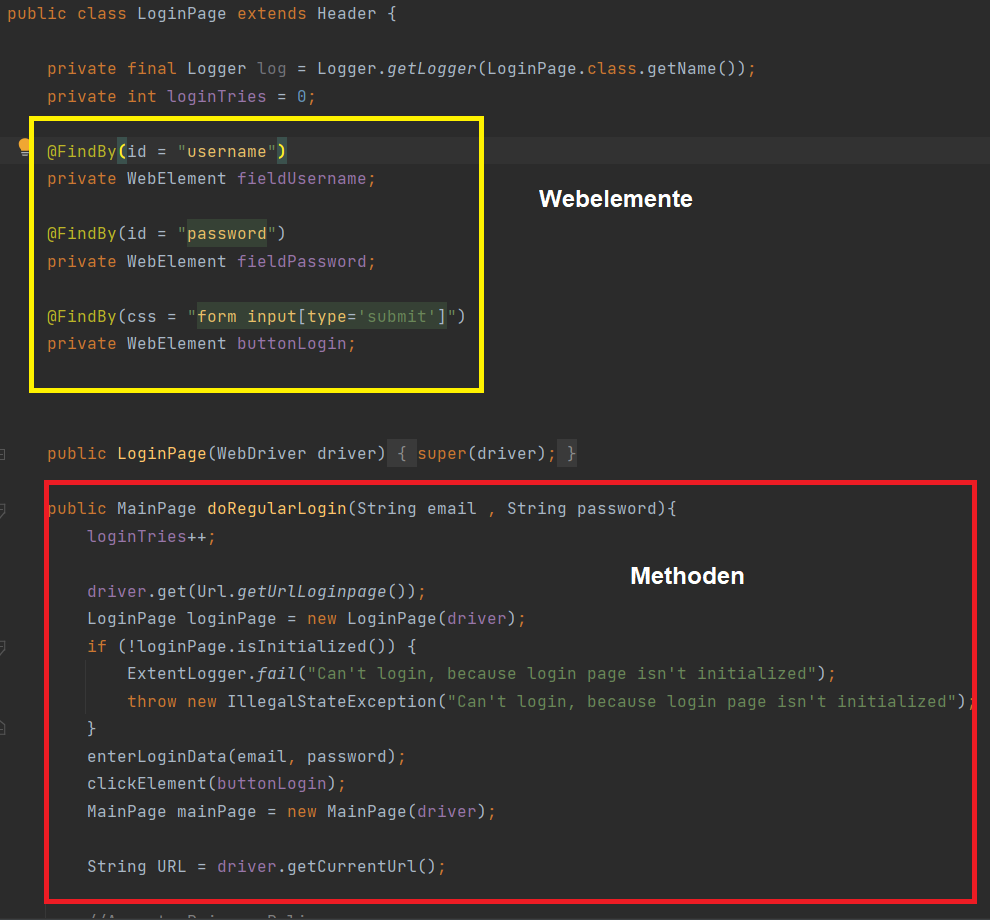
\includegraphics[scale=0.5]{images/page-example}
    \caption{Darstellung der jExam LoginPage mit dem Page Object Model} \label{fig:page-exp}
\end{figure}

\begin{figure}[H]
    \centering
    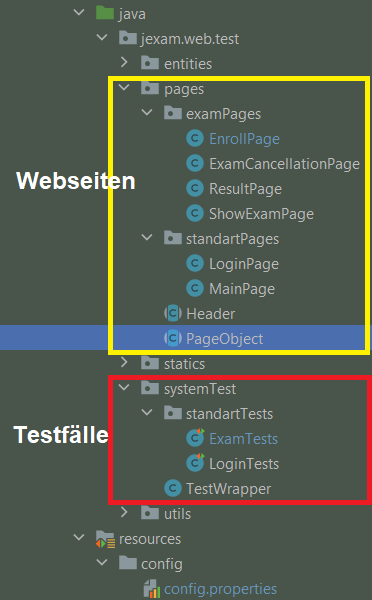
\includegraphics[scale=0.6]{images/page-object}
    \caption{Projektstruktur von jExam Page Object Model} \label{fig:page-obj}
\end{figure}

\subsubsection{Factory}

Page Factory ist eine Klasse, die von Selenium WebDriver bereitgestellt
wird, um das Page Object Model zu implementieren. Das Page Object
Repository wird mit Hilfe des Page Factory-Konzepts von den Testmethoden
getrennt. Page Factory bietet Annotationen, um Elemente zu initialisieren und sie
anschaulich und lesbar macht. Zu den Vorteilen seiner Verwendung gehören:

\begin{enumerate}
    \item \textbf{Sauberer Code}: Das definierte Webelement wird von den Methoden
    getrennt, um eine Webseite in einer Page Object sauber und
    aufgeräumt zu gestalten.
    \item \textbf{Lesbar und beschreibend}: Ein Webelement wird als Variable
    (bekannt als Object Field) deklariert, und die Field-Annotation
    (@FindBy siehe \Cref{fig:page-exp}) wird verwendet, um den Namen, den Typ und
    die Position des Elements zu beschreiben. Auf diese Weise können
    definierte Webelement anhand seiner Annotationen wie Name, Typ
    usw. leicht identifiziert werden.
    \item \textbf{Einfache Wartbarkeit}: Das definierte Webelement kann ohne
    Neudefinition überall in der Page Object Klasse und den Unterklassen
    verwendet werden. Das bedeutet, dass ein bestimmtes Webelement
    mehrmals verwendet werden kann, aber nur an einer Stelle
    definiert ist.
\end{enumerate}


Im nächsten Teil werden die Implementierung der Tests und die verwendeten
Methoden genauer beschrieben.





\subsection{Implementierung der Testsuite}

Das Schreiben eines UI-Tests mit Selenium ist ein Prozess, der je
nach der zu testenden Funktionalität mehr oder weniger lange dauert.
Je komplexer die Funktionalität ist, desto komplexer ist auch das
Schreiben des Tests. In diesem Kapitel geht es darum, den Prozess
der Testimplementierung zu beschreiben. Dazu wird ein Test verwendet,
der als Beispiel für die Beschreibung des Implementierungsprozesses
dienen soll : \textbf{Der Registrierungstest}. Dieser Test wurde ausgewählt,
weil er fast alle Funktionen abdeckt, die bei der Erstellung der
anderen Tests verwendet wurden. Das Schreiben von Tests ist in fünf
Phasen unterteilt:

\subsubsection{Phase 1: Initialisierung der Daten}

Vor der Durchführung von Tests ist es wichtig, die zu testende
Plattform mit Daten vorzubereiten. Dies ermöglicht es, die
Ausgangssituation der Plattform, die man testen möchte, zu
reproduzieren. Wenn beispielsweise die Verbindung eines Benutzers
mit einer Plattform getestet werden soll, ist es wichtig, dass die
Daten dieses Benutzers bereits in der Datenbank vorhanden sind.

Im aktuellen Fall wird dies von einem Docker-Container namens
Initializer (wird im Kapitel über Docker ausführlich behandelt)
durchgeführt, dessen Zweck  ist, ein Skript auszuführen, das Daten
in den JBoss-Server von jExam einspeist. Im Falle des
Registrierungstests wird eine gültige, aber nicht auf der
Plattform registrierte Matrikelnummer generiert (siehe \Cref{fig:testData}).

\begin{figure}[H]
    \centering
    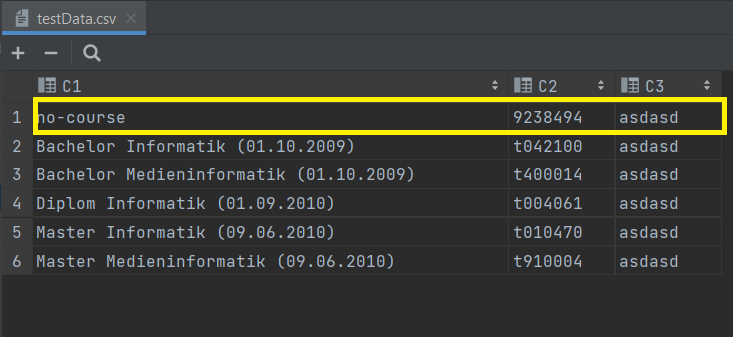
\includegraphics[scale=0.7]{images/testData}
    \caption{Vom Initializer erzeugte CSV-Daten} \label{fig:testData}
\end{figure}
\subsubsection{Phase 2: Erstellung eines Testszenarios}

In dieser Phase muss der Tester ein Ausführungsszenario für seinen 
Test erstellen. Es geht darum, die zu testende Funktion manuell
auf der Plattform auszuführen und die Ausführungsschritte zu 
dokumentieren, die in den nächsten Schritten automatisch wiederholt
werden. Dieser Prozess könnte auch in schriftlicher Form erfolgen
(normalerweise bei langen Szenarien). Diese Phase dient dazu, den 
Test im Detail zu planen und so die spätere Umsetzung zu erleichtern.
Im Falle des Registrierungstests ist das Szenario wie folgt festgelegt:

\begin{enumerate}
    \item Gehen Sie auf die Login-Seite und füllen Sie das Formular mit
    der nicht registrierten Matrikelnummer aus.
    \item Klicken Sie auf den Login-Button und Sie werden zur
    Registrierungsseite weitergeleitet.
    \item Füllen Sie das Registrierungsformular aus und klicken Sie
    auf Registrieren.
    \item Weiterleitung zur Seite Privacy Policy und Zustimmung zu
    den allgemeinen Nutzungsbedingungen
    (prüfen Sie, ob der TestUser automatisch eingeloggt wird).
    \item Logout und Login erneut mit den Zugangsdaten und der
    Matrikelnummer, die Sie bei der Registrierung verwendet haben.
    \item Wenn alles richtig funktioniert: Die Registrierung war erfolgreich.
\end{enumerate}
\subsubsection{Phase 3: Erstellung von Objekt-Seiten}

Wie bereits im \autoref{subsec:entwurfsmuster} erwähnt, wird das Object
Page Entwurfsmuster für die Erstellung von Tests verwendet.
Vor der Implementierung des Szenarios muss der Tester zunächst
die Objekte und Seiten erstellen, die für die Ausführung des Szenarios
erforderlich sind. Im Rahmen des Registrierungstests müssen folgende
Seiten erstellt werden: LoginPage, RegistrationPage, ContractPage
(Privacy Policy) und die MainPage. Wenn die RegistrationPage
im Detail betrachtet wird, kann man feststellen, dass diese
Java-Klasse (wie alle anderen Object-Seiten) einige besondere Merkmale
aufweist.

Zunächst erbt sie von der Klasse Header (die den auf allen Seiten
vorhandenen Header repräsentiert). Der Header selbst stammt von
PageObject ab, das die Grundstruktur einer Seite repräsentiert
(siehe \Cref{fig:pag-uml}). Die Klassen Header und PageObject enthalten
Webelelemente und Methoden, die normalerweise auf allen Seiten der
Anwendung zugänglich sind. Dadurch kann das Design Pattern Page
Object optimal genutzt werden.

\begin{figure}[H]
    \centering
    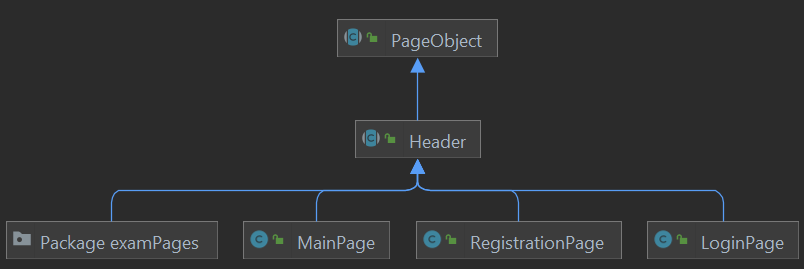
\includegraphics[scale=0.7]{images/pag-uml}
    \caption{UML Diagramm für die Java Page-Objekte} \label{fig:pag-uml}
\end{figure}

Zweitens enthält die Registrationpage eigene Webelemente.
Zum Beispiel die verschiedenen Inputs des auszufüllenden Formulare und
die anzuklickenden Bestätigungsbuttons (siehe Quellcode \ref{lst:registerpage}). Darüber hinaus
verfügt die Seite über die Methode registerUser, die ein
Formularobjekt (RegistrationForm) als Parameter hat und alle Eingaben
des Formulars ausfüllt und die ContractPage zurückgibt.

\begin{lstlisting}[label={lst:registerpage}, caption={RegistrationPage Quellcode}]
// RegistrationPage.java

    public class RegistrationPage extends Header {

    @FindBy(id = "cfirstname")
    private WebElement fieldFirstName;

    @FindBy(id = "csurname")
    private WebElement fieldName;

    @FindBy(id = "cmatrikel")
    private WebElement matrikel;

    public RegistrationPage(WebDriver driver) {
        super(driver);
    }

    @Override
    public boolean isInitialized() {
        WebElement h1_title;
        try{
            h1_title = driver.findElement(By.xpath("//H1[text()='Registrierung']"));
        }catch (NoSuchElementException e ){
            ExtentLogger.info("Main Title was not found");
            return false;
        }
        return h1_title.isDisplayed();
    }


    public ContractPage registerUser(RegistrationForm registrationForm){

        sendKeysToElement(fieldFirstName, registrationForm.firstName);
        sendKeysToElement(fieldName, registrationForm.lastName);

        Select fieldGender = new Select(driver.findElement(By.id("cgender")));
        fieldGender.selectByValue(registrationForm.gender);

        Select fieldCountry = new Select(driver.findElement(By.id("ccountry")));
        fieldCountry.selectByValue(registrationForm.country);

        Select fieldLanguage = new Select(driver.findElement(By.id("clanguage")));
        fieldLanguage.selectByValue(registrationForm.defaultLanguage);


        matrikel.clear();
        sendKeysToElement(matrikel, registrationForm.matrikel);

        Select fieldFaculty = new Select(driver.findElement(By.id("ou-combo")));
        fieldFaculty.selectByValue(registrationForm.faculty);

        Select fieldDegree = new Select(driver.findElement(By.id("degree-combo")));
        fieldDegree.selectByValue(registrationForm.degree);

        Select fieldExamReg = new Select(driver.findElement(By.id("er-combo")));
        fieldExamReg.selectByValue(registrationForm.examRegulation);

        WebElement addFaculty = driver.findElement(By.id("addEr"));

        clickElement(addFaculty);

        WebElement validationBtn = driver.findElement(By.xpath("(//INPUT[@class='btn fill-primary'])[2]"));
        clickElement(validationBtn);

        return new ContractPage(driver);
    }
}
\end{lstlisting}
\subsubsection{Phase 4: Erstellen von Verbindungen zwischen den Seiten}

Wenn auf einen Link geklickt oder einfach ein Formular bestätigt wird,
wird man normalerweise auf eine andere Seite weitergeleitet. Diese Phase
befasst sich im Wesentlichen mit der Umsetzung dieser Aufgabe.
Im Rahmen der Implementierung des Registrierungstests geht es darum,
die Seiten zwischen zwei Aktionen miteinander zu verbinden.
Zum Beispiel sollte die Registrierungsfunktion nach einem Klick
auf den Button Login die RegisterPage zurückgeben (siehe \Cref{fig:reg-page}).
Dies ist in der Tat eine Modellierung der Web-Navigation in Java.
Diese Arbeit muss durchgeführt werden und macht in der letzten Phase
Sinn.

\begin{figure}[H]
    \centering
    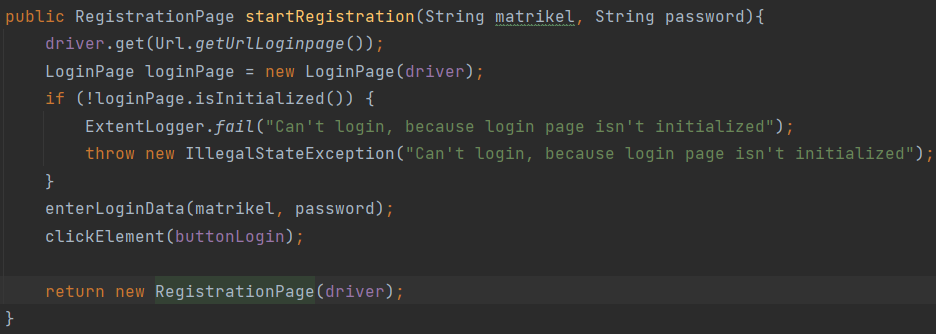
\includegraphics[scale=0.5]{images/reg-page}
    \caption{StartRegistration Funktion} \label{fig:reg-page}
\end{figure}

\subsubsection{Phase 5: Implementierung der tests nach dem szenario}

Diese Phase konzentriert sich auf die Umsetzung des in Phase 2
beschriebenen Szenarios. Es handelt sich um das Schreiben des Tests
an sich. In dieser Phase wird der Tester die Aktionen eines Nutzers
nacheinander ausführen.

Im Fall des Registrierungstests geht es zunächst darum, sich mit einer
Matrikelnummer zu registrieren, die nicht in der Datenbank verzeichnet
ist. Dann wird das Registrierungsformular mit den zuvor festgelegten
Daten ausgefüllt. Im nächsten Schritt werden die Allgemeinen
Geschäftsbedingungen akzeptiert und der Testuser dann einloggt.
Um zu überprüfen, ob die Registrierung erfolgreich war, muss der
Tester einen Login-Test mit den Daten simulieren, die er bei der
Registrierung verwendet hat (siehe Quellcode \ref{lst:reg-test}). Zwischen all
diesen Schritten werden Verifikationsprozesse durchgeführt
(z. B. ob eine Seite korrekt initialisiert wurde).

Es ist wichtig, Logs und ExtentLogger zu verwenden, um jeden Schritt
der Tests zu dokumentieren. Dadurch kann bei der Erstellung des
Ausführungsberichts nachvollzogen werden, welche Schritte während
des Tests durchgeführt wurden. Außerdem können diese Logs zeigen,
ob die Tests abgeschlossen wurden oder ob während der Ausführung
ein Fehler aufgetreten ist.


\begin{lstlisting}[label={lst:reg-test}, caption={Registration Test Quellcode}]

    // Registration Test Quellcode

    @Test
    @Description("New User Registration")
    public void doRegistrationTest(){
        ExtentReport.createTest("Test User Registration");
        ExtentLogger.info("⛔⛔ If you dont see \"Test Passed\" at the end, the Test didn't passed !");

        TestUser user = TestUser.REGISTRATION_USER;
        RegistrationPage registrationPage = startRegistration(user.username, user.password);
        Assert.assertTrue(registrationPage.isInitialized(),"Registrationpage was not correctly initialized");
        ExtentLogger.info("Registration Page is correctly initialized !");

        RegistrationForm form = new RegistrationForm(user.username+"@", user.username+"@", "f",
                "DE", user.username, "30010", "Bachelor Informatik", "1533186");
        ContractPage contractPage = registrationPage.registerUser(form);
        Assert.assertTrue(contractPage.isInitialized(), "Contractpage should be initialized !");
        ExtentLogger.info("Contract Page is initialized");

        MainPage mainPage = contractPage.acceptPrivacyPolicy();
        ExtentLogger.info("Privacy Policy was accepted");

        ExtentLogger.info("Try logout and login !");
        LoginPage loginPage = mainPage.selectLogoutLink();
        Assert.assertTrue(loginPage.isInitialized() , "Expected to land on login page, after log in, but landed on another page");
        ExtentLogger.info("Logout was successful, got on login page");
        log.info("Logout was successful, got on login page");

        // New Login with New Identifier
        mainPage = regularLogin(user.username , user.password);
        Assert.assertTrue(mainPage.isInitialized() , "Expected to land on main page, after log in, but landed on another page");
        ExtentLogger.info("Login was successful, got on main page");
        log.info("Login was successful, got on main page");

        loginPage = mainPage.selectLogoutLink();
        Assert.assertTrue(loginPage.isInitialized() , "Expected to land on login page, after log in, but landed on another page");
        ExtentLogger.info("Logout was successful, got on login page");
        log.info("Logout was successful, got on login page");

        ExtentLogger.info("Registration was successful");
        log.info("Registration was successful");
        ExtentLogger.pass("Test passed");
    }
\end{lstlisting}

Es gibt noch viele weitere Funktionen und Klassen, die in dieser
Arbeit nicht beschrieben werden können. Die Details des Schreibens
und aller Funktionen werden jedoch in der Dokumentation der
Testinfrastruktur ausführlich erläutert.

\subsection{Erreichte Ergebnisse}

\subsection{Docker}

Bei der Entwicklung einer Anwendung gibt es einige Probleme, die
sehr oft während der Entwicklung oder sogar während der Produktion
auftreten. Diese Probleme werden oft durch die folgenden Aussage
formuliert:

\begin{enumerate}
    \item Das Skript funktionierte gestern aber heute nicht mehr.
    \item Das Skript funktioniert auf diesem Rechner und nicht auf
    dem Rechner eines Kollegen/Kunden.
    \item Das Skript funktioniert nur mit Java 5 und nicht mit Java 8.
    \item Die Anwendung muss in allen aktuellen Browser-Versionen von Chrome (80,81,82,\ldots,89) und Firefox (78,79,80,\ldots,84) getestet werden.
    Mussen die alle installiert werden ?
\end{enumerate}

Docker ist eine Open-Source-Containerisierungsplattform. Sie
ermöglicht es Entwicklern, Anwendungen in \gls{container}
(standardisierte ausführbare Komponenten) zu verpacken.
Sie kombinieren den Quellcode der Anwendung mit den
Betriebssystembibliotheken und Abhängigkeiten, die für die
Ausführung dieses Codes in jeder Umgebung erforderlich sind.
Container vereinfachen die Bereitstellung verteilter Anwendungen und
erfreuen sich zunehmender Beliebtheit (vgl. \cite{docker}).

Docker macht das Erstellen, Bereitstellen und Verwalten von
Containern leichter, einfacher und sicherer (vgl. \cite{ibm-docker}).
Docker ist im Wesentlichen ein Toolkit, das es Entwicklern ermöglicht,
Container mit einfachen Befehlen und arbeitssparender Automatisierung
über eine einzige API zu erstellen, bereitzustellen, auszuführen,
zu aktualisieren und zu beenden (vgl. \cite{ibm-docker}). Zu den Vorteilen der Verwendung von
Docker gehören :

\begin{itemize}
    \setlength\itemsep{1em}
    \item[] \textbf{Portabilität}: Ein Container erstellt ein ausführbares
    Softwarepaket, das vom Host-Betriebssystem abstrahiert
    (nicht an dieses gebunden oder von diesem abhängig ist)
    und daher portabel und in der Lage ist, auf jeder Plattform oder
    Cloud einheitlich und konsistent zu laufen.

    \item[] \textbf{Agilität}: Docker für die Ausführung von Containern hat den
    Industriestandard für Container mit einfachen Entwicklertools
    und einem universellen Paketierungsansatz geschaffen, der sowohl
    unter Linux- als auch unter Windows-Betriebssystemen funktioniert.
    Das Container-\"Okosystem hat sich auf Engines verlagert, die von
    der Open Container Initiative (OCI) verwaltet werden.
    Softwareentwickler können weiterhin agile oder DevOps-Tools
    und -Prozesse für eine schnelle Anwendungsentwicklung und
    -verbesserung verwenden.

    \item[] \textbf{Geschwindigkeit}: Container werden oft als leichtgewichtig
    bezeichnet, was bedeutet, dass sie den Betriebssystemkern des
    Rechners gemeinsam nutzen und nicht mit diesem zusätzlichen
    Overhead belastet werden. Dies steigert nicht nur die Effizienz
    des Servers, sondern senkt auch die Server- und Lizenzkosten und
    verkürzt die Startzeiten, da das Betriebssystem nicht gebootet
    werden muss.

    \item[] \textbf{Isolierung von Fehlern}: Jede containerisierte Anwendung ist
    isoliert und arbeitet unabhängig von den anderen. Der Ausfall
    eines Containers hat keine Auswirkungen auf den weiteren Betrieb
    der anderen Container. Entwicklungsteams können alle technischen
    Probleme innerhalb eines Containers identifizieren und beheben,
    ohne dass es zu Ausfallzeiten in anderen Containern kommt.
    Außerdem kann die Container-Engine alle
    Sicherheitsisolationstechniken des Betriebssystems nutzen, um Fehler innerhalb der
    Container zu isolieren.

    \item[] \textbf{Effizienz}: Software, die in containerisierten Umgebungen
    ausgeführt wird, teilt sich den Betriebssystemkern des Rechners,
    und Anwendungsschichten innerhalb eines Containers können von
    mehreren Containern gemeinsam genutzt werden. Daher haben
    Container von Natur aus eine geringere Kapazität als eine VM
    und benötigen weniger Anlaufzeit, so dass weitaus mehr Container
    auf der gleichen Rechenkapazität wie eine einzelne VM ausgeführt
    werden können. Dies führt zu einer höheren Server-Effizienz und
    senkt die Server- und Lizenzierungskosten.

    \item[] \textbf{Sicherheit}: Die Isolierung von Anwendungen in Form von
    Containern verhindert von Natur aus, dass bösartiger Code in
    andere Container oder das Hostsystem eindringt. Darüber hinaus
    können Sicherheitsberechtigungen definiert werden, um unerwünschte
    Komponenten automatisch am Eintritt in Container zu hindern oder
    die Kommunikation mit unnötigen Ressourcen einzuschränken.

\end{itemize}


Docker bietet also die Möglichkeit, ein Werkzeug zu bauen, das auf
allen Arten von Systemen unabhängig von den lokalen Konfigurationen
der einzelnen Benutzer funktioniert. Es spielt also keine Rolle,
welche Java-Version oder welches Betriebssystem ein Benutzer hat (vgl. \cite{ibm-docker}).
Anstatt eine Vielzahl von Abhängigkeiten herunterzuladen und zu
installieren, kann man auch einfach einen Container mit allen
notwendigen Abhängigkeiten erstellen und ihn auf jedem System
verwenden, das Docker unterstützt. Die Verwendung von Docker wird all diese Vorteile für die Entwicklung
der Testinfrastruktur nutzen. Das zusätzliche Werkzeug zur
Orchestrierung der verschiedenen Container ist jedoch Docker-compose.


Wenn Sie eine Anwendung aus Prozessen in mehreren Containern erstellen,
die sich alle auf demselben Host befinden, können Sie Docker-Compose
verwenden, um die Anwendungsarchitektur zu verwalten. Docker Compose
erstellt eine YAML-Datei, die die Dienste angibt, die in der Anwendung
enthalten sein sollen, und kann die Container mit einem einzigen
Befehl bereitstellen und ausführen. Mithilfe von Docker Compose ist
es möglich, persistente Volumes für den Speicher zu definieren,
Basisknoten anzugeben und die Abhängigkeiten der Dienste zu
dokumentieren und zu konfigurieren.


Im nächsten Kapitel wird beschrieben, wie Docker und Docker-Compose
für die Einrichtung der Testinfrastruktur von jExam verwendet
wurden.



